\chapter{Administrer l'application}

\section{Gérer les droits}
\label{droits}

Depuis la version 1.1, les scripts de création des bases de données intègrent la génération initiale des groupes et des droits associés, ceci afin de faciliter la phase de mise en route.

Toutefois, vous devrez créer des groupes d'utilisateurs correspondant à vos projets, et modifier ensuite les projets pour donner les droits adéquats aux groupes créés (\textit{cf.} \ref{projet}, page \pageref{projet}).

\subsection{Principe général}

Les droits sont gérés selon le principe initialement utilisé dans la bibliothèque PHPGACL \cite{phpgacl}, aujourd'hui obsolète. 

Les logins sont déclarés dans des groupes organisés de manière hiérarchique : un groupe hérite des droits attribués à ses parents.

Les droits utilisés dans le logiciel sont associés à des groupes. Il est possible d'attribuer plusieurs droits à un même groupe, et un droit peut être détenu par des groupes différents.

Si le paramètre \textit{\$LDAP["groupSupport"]} est positionné à \textit{true}, les groupes dont fait partie le compte LDAP sont également récupérés. Si ces groupes se voient attribués des droits, les comptes associés les récupéreront automatiquement.

Voici le schéma des tables utilisées pour gérer les droits :

\begin{figure}[H]
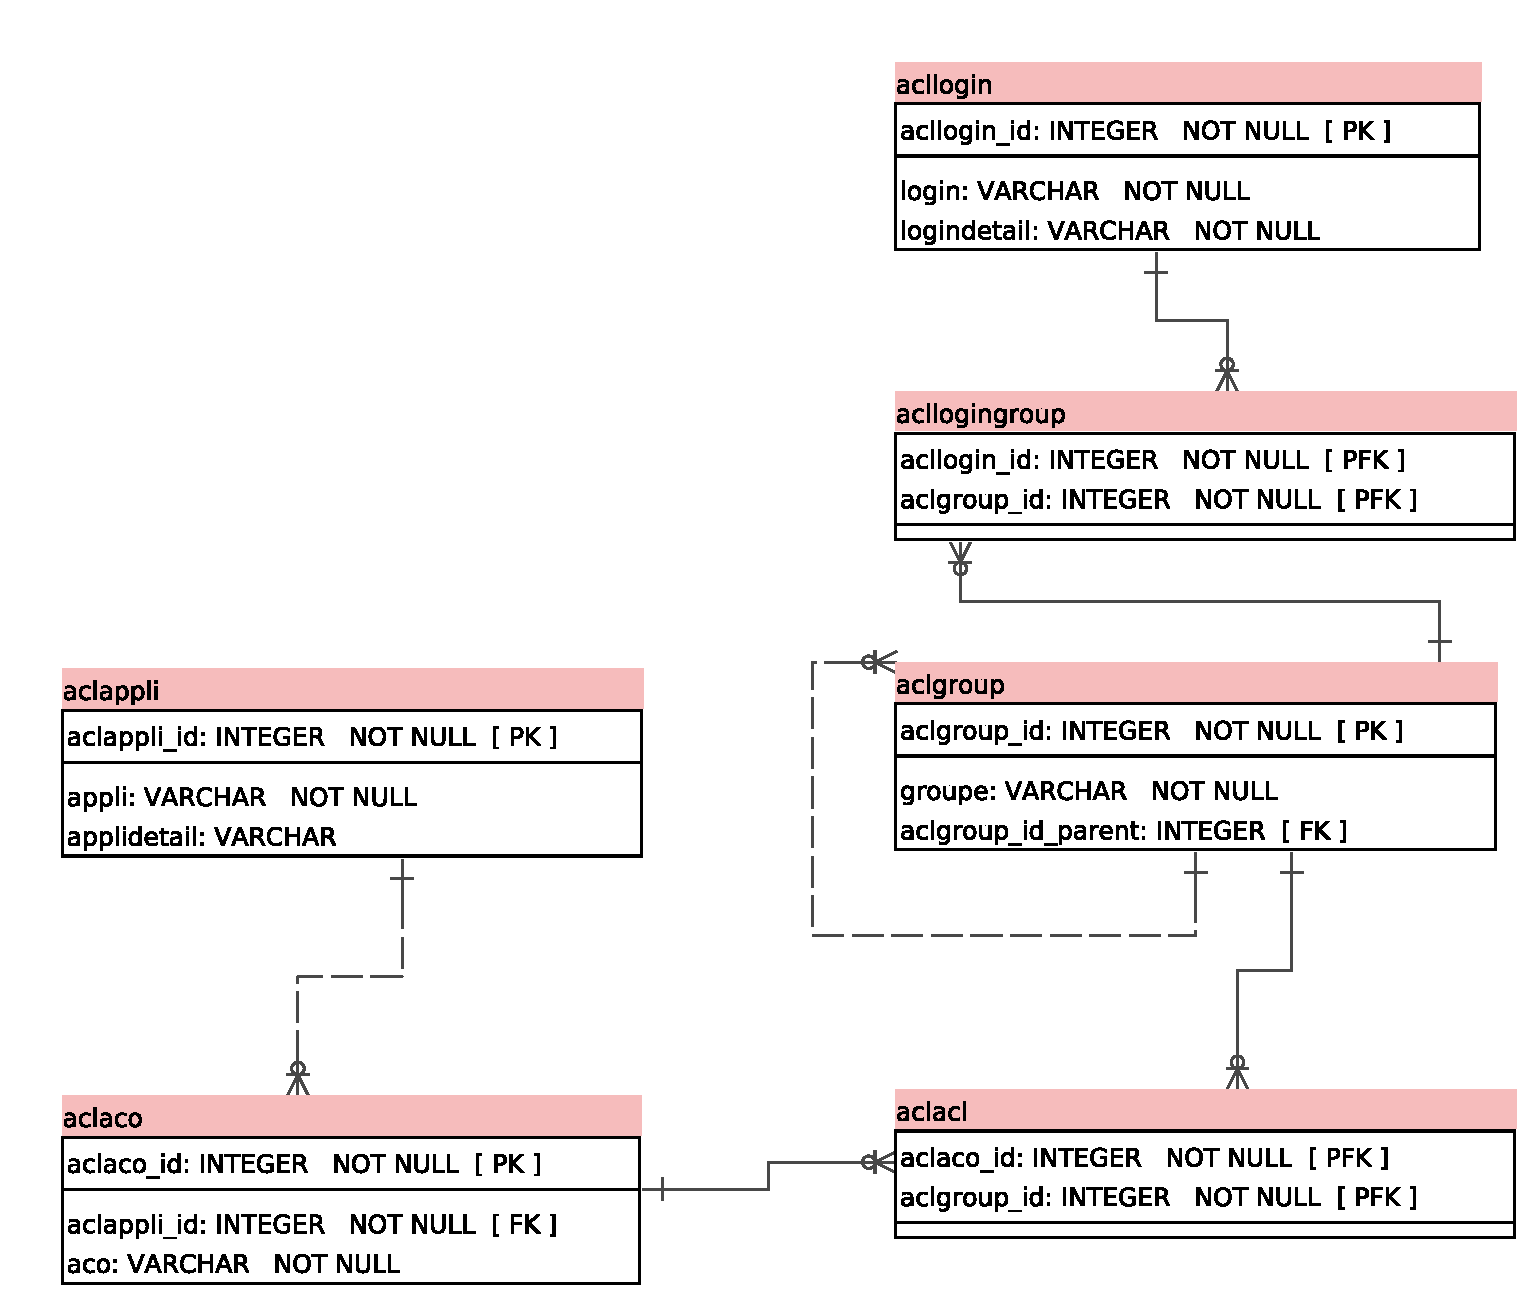
\includegraphics[width=\linewidth]{images/acl_only}
\caption{Schéma des tables utilisées pour gérer les droits}
\end{figure}

Voici la description des tables :
\begin{description}
\item[acllogin] : liste des logins utilisés. Si un compte est créé dans la base locale d'identification, un enregistrement est également créé dans cette table. Pour les identifications LDAP ou CAS, ils doivent être identiques. Si seuls les groupes LDAP sont utilisés pour un compte, il n'a pas besoin d'être décrit ici ;
\item[aclappli] : liste des applications gérées. Il est possible de gérer, à partir de la même base de données, plusieurs ensembles de droits, qui utilisent les mêmes logins.
\item[aclaco] : liste des droits déclarés dans l'application ;
\item[aclgroup] : liste des groupes contenant les logins, et qui détiennent les droits. Un groupe peut hériter d'un autre groupe. Les droits associés au groupe parent sont également attribués au groupe hérité ;
\item[acllogingroup] : table permettant de déclarer les logins associés à un groupe ;
\item[aclacl] : table décrivant les droits détenus par un groupe.
\end{description}

Le module d'administration permet de saisir toutes ces informations. Il faut que l'utilisateur dispose du droit \textit{admin}, c'est à dire qu'il fasse partie du groupe \textit{admin} (configuration par défaut à l'initialisation de la base des droits) pour pouvoir accéder à ces fonctions.

\subsection{Créer un nouvel utilisateur}

Les utilisateurs peuvent être issus soit de l'annuaire LDAP, soit de la base interne. 
Pour créer un nouvel utilisateur dans la base locale :
\begin{itemize}
\item \textit{Administration $\rightarrow$ Liste des comptes }
\item \textit{Nouveau login}
\item renseignez au minimum le login.
\end{itemize}

\begin{figure}[H]
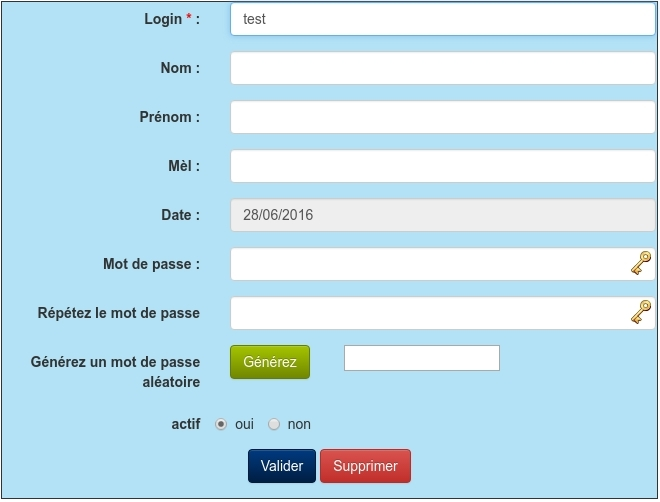
\includegraphics[width=\linewidth]{images/user_create}
\caption{Écran de saisie d'un login de connexion}
\end{figure}

Pour créer le mot de passe, vous pouvez cliquer sur le bouton \textit{Générez}, qui  en générera un automatiquement. Envoyez-le par mél à son destinataire (par \textit{copier-coller}), en lui demandant de le modifier à la première connexion (icône en forme de clé, dans le bandeau, en haut à droite).

Les mots de passe doivent respecter les règles suivantes :
\begin{itemize}
\item ils doivent avoir une longueur minimale de 8 caractères ;
\item ils doivent comprendre trois types de caractères différents parmi les minuscules, majuscules, chiffres et caractères de ponctuation ;
\item ils ne peuvent pas être réutilisés pour le même login ;
\item les mots de passe n'expirent pas.
\end{itemize}

Les mots de passe sont stockés sous forme d'empreinte, calculée en rajoutant un sel\footnote{chaîne de caractère rajoutée au mot de passe -- en général le login ou un identifiant -- qui permet d'éviter que deux mots de passe identiques, associés à deux logins différents, aient la même empreinte} et encodés en SHA256 : ils ne peuvent pas être retrouvés en cas de perte.

L'application n'intègre pas de module permettant de régénérer automatiquement un mot de passe en cas de perte : c'est au responsable applicatif d'en fournir un nouveau.

La création d'un compte entraîne la création d'une entrée identique dans la table des \textit{acllogin}, utilisée pour attribuer les droits.

Pour désactiver temporairement un compte, sélectionnez \textit{non} dans la zone \textit{actif}. Si le compte ne doit plus être utilisé, supprimez-le.

Attention : si le compte disposait des droits d'administration, assurez-vous que vous avez toujours un compte disposant des mêmes droits avant la suppression.

\subsection{Créer un login utilisé dans la gestion des droits}

Indépendamment du compte de connexion, qui peut être soit issu de la base interne, soit récupéré auprès d'un annuaire LDAP ou d'un serveur CAS, l'application a besoin de connaître les utilisateurs pour pouvoir leur attribuer des droits.

À partir du menu, choisissez \textit{Administration $\rightarrow$ ACL - logins}.

Vous pouvez modifier un login existant ou en créer un nouveau. Dans ce cas, vous devrez indiquer au minimum le login utilisé (identique à celui qui est employé pour la connexion à l'application : base de données interne, annuaire LDAP, serveur CAS).

\begin{figure}[H]
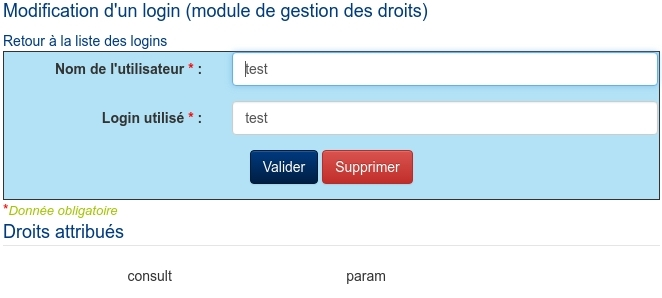
\includegraphics[width=\linewidth]{images/acl_login}
\caption{Écran de modification d'un login dans le module de gestion des droits}
\end{figure}


Sous l'écran de saisie figurent la liste des droits attribués à un login (en modification, le calcul n'est réalisé qu'à l'affichage de la page).

\subsection{Définir les groupes d'utilisateur}

Les groupes d'utilisateurs sont gérés selon un mécanisme d'héritage. Un groupe de haut niveau hérite des groupes précédents : si des droits ont été attribués à un groupe de niveau inférieur, un login associé à un groupe de niveau supérieur les récupère également.

Pour définir les groupes, dans le menu, choisissez \textit{Administration $\rightarrow$ ACL - groupes de logins}.

\begin{figure}[H]
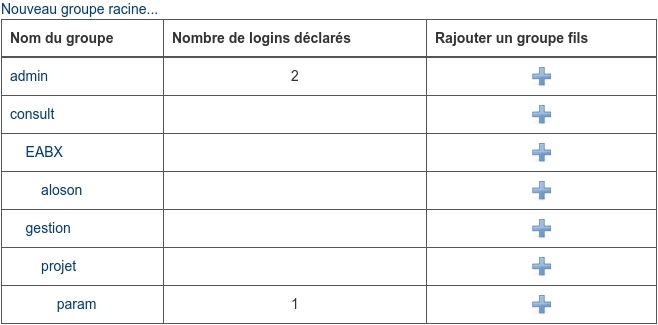
\includegraphics[width=\linewidth]{images/acl_groupe}
\caption{Liste des groupes de logins}
\end{figure}

Ainsi, le login déclaré dans le groupe \textit{param} récupérera les droits attribués aux groupes \textit{projet}, \textit{gestion} et \textit{consult}.

Pour créer un groupe, deux possibilités :
\begin{itemize}
\item soit le groupe est à la base d'une nouvelle branche : utilisez alors \textit{Nouveau groupe racine...} ;
\item soit le groupe hérite d'un autre groupe : cliquez sur le signe + (\textit{Rajouter un groupe fils}).
\end{itemize}

Vous pouvez indiquer les logins qui sont rattachés à ce groupe.


\subsection{Créer une application}
Le moteur utilisé pour faire fonctionner le logiciel COLLEC permet de gérer des droits différents pour des jeux de données différents, à partir du même code applicatif. Chaque couple \textit{logiciel} $\leftrightarrow$ \textit{base de données} constitue donc une \textit{application}, au sens de la gestion des droits.

Il est ainsi possible, à partir de la même base de données, de définir des droits différents selon les jeux de données utilisés (un jeu de données correspond à un schéma de base de données comprenant l'intégralité des tables applicatives).

À partir du menu, choisissez \textit{Administration $\rightarrow$ ACL - droits} :
\begin{figure}[H]
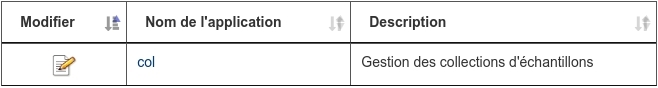
\includegraphics[width=\linewidth]{images/liste_appli}
\caption{Liste des applications déclarées}
\end{figure}

Pour créer une nouvelle application, choisissez \textit{Nouvelle application...}. 

\begin{figure}[H]
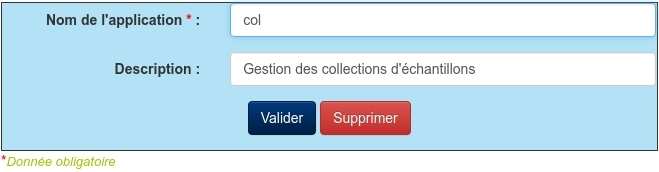
\includegraphics[width=\linewidth]{images/appli_change}
\caption{Écran de saisie d'une application}
\end{figure}

Le nom de l'application doit impérativement correspondre à la valeur \textit{\$GACL\_appli} dans les fichiers de paramètres : c'est ce qui permet au framework de savoir quels droits appliquer.

\subsection{Définir les droits utilisables dans l'application}

À partir de la liste des applications, cliquez sur le nom de celle pour laquelle vous voulez définir les droits utilisables. 
À partir de la liste, sélectionnez \textit{Nouveau droit...}.

\begin{figure}[H]
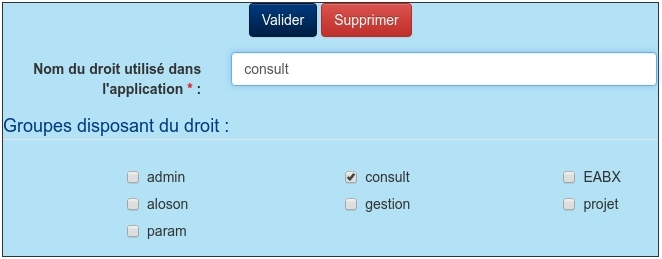
\includegraphics[width=\linewidth]{images/appli_droit}
\caption{Écran de saisie des droits associés à une application}
\label{applidroit}
\end{figure}

Le nom du droit doit être celui défini dans le corps de l'application (les droits sont positionnés dans les fichiers \textit{param/actions.xml}, qui contient la liste des modules utilisables, et \textit{param/menu.xml}, qui sert à générer le menu -- \textit{cf.} table \ref{droitsCollec} \textit{\nameref{droitsCollec}}, page \pageref{droitsCollec}).

Indiquez les groupes d'utilisateurs qui seront associés au droit courant.

\subsection{Cas particulier des groupes et des logins issus d'un annuaire LDAP}

Si vous avez paramétré l'application pour qu'elle s'appuie sur un annuaire LDAP pour gérer l'affectation des utilisateurs dans les groupes, vous n'êtes pas obligés de les déclarer explicitement dans le module de gestion des droits.

\subsubsection{Droits attribués à un groupe LDAP}

Tous les utilisateurs d'un groupe héritent d'un droit dans l'application.

\begin{itemize}
\item définissez le nom du groupe (en respectant la casse) dans le tableau des groupes d'utilisateurs (par exemple, EABX) ;
\item sélectionnez le nom de ce groupe dans les droits utilisables ;
\item tous les utilisateurs de l'annuaire LDAP récupéreront automatiquement les droits attribués à ce groupe.
\end{itemize}

\subsubsection{Droits attribués à un utilisateur particulier de l'annuaire LDAP}

Un utilisateur s'identifie auprès de l'annuaire LDAP, mais dispose de droits particuliers.

\begin{itemize}
\item créez son login dans la gestion des droits ;
\item rajoutez-le dans le groupe d'utilisateurs adéquat.
\end{itemize}


\section{Droits spécifiques de l'application COLLEC}

\subsection{Droits à positionner}
Voici les droits nécessaires pour faire fonctionner correctement l'application :

\begin{longtable}{|p{5cm}|p{10cm}|}
\hline
\textbf{Droit} & \textbf{Usage} \\
\hline
\endhead
admin &	Gestion des utilisateurs et des droits\\
\hline
param &	Définition des tables de paramètres généraux, gestion d'un projet\\
\hline
projet &	rajout des types d'échantillons ou de conteneurs, import de masse \\
\hline
gestion &	Ajout d'un échantillon pour les projets autorisés, entrée/sortie. Droit attribué par défaut si l'utilisateur fait partie d'au moins un projet \\
\hline
consult	& Consultation des informations, sans possibilité de modification. Le droit de consultation doit être indiqué volontairement\\
\hline

\caption{\label{droitsCollec}Liste des droits utilisés}
\end{longtable}

Ces droits doivent être définis pour chaque application (couple \textit{logiciel} $\leftrightarrow$ \textit{base de données}) gérée par la base de gestion des droits.

\subsection{Gestion des projets}
\label{projet}

Les échantillons étant obligatoirement rattachés à un projet, vous devrez en créer au minimum un à partir du menu d'administration. Un utilisateur avec les droits de gestion ne peut modifier que les échantillons pour lesquels il est autorisé (les projets qui sont rattachés au groupe dont il fait partie).

Voici le principe de gestion des droits pour les projets :
\begin{itemize}
\item Dans \textit{Administration} > \textit{ACL - Groupes de logins}, déclarez les groupes adéquats. En cas d'utilisation des groupes LDAP, les saisir avec la même casse que dans l'annuaire (EABX p. e.).

Il est possible de définir une hiérarchie des groupes, quelle que soit l'origine de l'affectation (base de données ou annuaire Ldap).
Dans le cas où l'annuaire Ldap n'est pas utilisé pour gérer les groupes, renseignez les logins en face des groupes dans le même écran ;
\item Dans les projets, sélectionnez les groupes autorisés (\textit{cf.} \ref{applidroit} \textit{\nameref{applidroit}}, page \pageref{applidroit}) ;
\item les utilisateurs faisant partie des groupes autorisés disposeront des droits de \textit{gestion} pour le projet considéré.
\end{itemize}

\section{Configurer les paramètres généraux}
\label{param}
L'ensemble des paramètres sont accessibles à partir du menu \textit{Paramètres}. 

Par défaut, tous les utilisateurs qui disposent du droit de consultation peuvent visualiser les paramètres. La modification n'est possible que pour ceux qui disposent des droits suivants :

\begin{longtable}{|p{4cm}|p{8cm}| p{3cm}|}
\hline
\textbf{Nom} & \textbf{Description} & \textbf{Droit nécessaire} \\
\hline
\endhead
Projets & Liste des projets et droits associés & admin \\
\hline
Protocoles & Protocoles de prélèvement des échantillons & projet \\
\hline
Opérations & Opérations rattachées aux protocoles & projet \\
\hline
Type d'événement & Événements survenant aux objets & param \\
\hline
Familles de conteneurs & Mécanisme pour retrouver les conteneurs selon leur nature (pièce, caisse...) & param, projet\\
\hline
Conditions de stockage & Mécanisme de conservation (lyophilisation, p. e.) & param, projet\\
\hline
Motifs de déstockage & Raisons invoquées pour sortir un objet du stock & param, projet\\
\hline
Types de conteneurs & Modèles de conteneurs (porteurs des étiquettes, entre autres) & param, projet\\
\hline
Statut des objets & Liste des statuts que peut prendre un objet & param\\
\hline
Type d'échantillon & Modèles des échantillons (rattachables à un type de conteneur) &  param, projet\\
\hline
Sous-échantillonnage & Pour les échantillons composés d'éléments indifférenciables, unité utilisée pour réaliser le sous-échantillonnage (nombre, volume...) & param \\
\hline
Étiquettes & Modèles des étiquettes imprimables & param \\
\hline
Types d'identifiants & Types d'identifiants complémentaires des objets & param \\
\hline

\caption{Liste des paramètres et droits de modification associés}
\end{longtable}

\section{Créer ou modifier un modèle d'étiquettes}

\begin{figure}[H]
\centering
\fbox{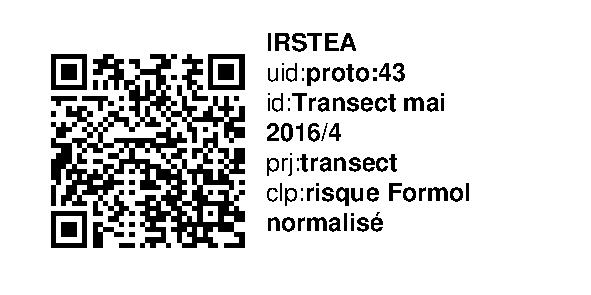
\includegraphics{images/etiquette}}
\caption{Exemple d'étiquette}
\end{figure}

Les étiquettes sont créées en recourant au logiciel FOP \cite{fop}, écrit en Java. Voici les opérations réalisées par l'application pour générer les étiquettes :
\begin{itemize}
\item pour chaque objet concerné (des containers ou des échantillons associés à un type de container, et si le type de container est rattaché à un modèle d'étiquettes), une image du QRcode est générée dans le dossier \textit{temp} ;
\item dans le dossier \textit{temp}, un fichier au format XML est généré, contenant les informations à imprimer sur l'étiquette ;
\item un fichier au format XSL, qui contient les ordres de création de l'étiquette, est également créé dans le même dossier. Le contenu de ce fichier est issu d'un enregistrement provenant de la table \textit{label} ;
\item le programme PHP fait appel à FOP pour générer, à partir du fichier XML et en utilisant le fichier XSL, un fichier PDF. Une page du fichier correspond à une étiquette (mécanisme utilisé par les imprimantes à étiquettes pour les séparer).
\end{itemize}

La configuration du modèle d'étiquettes revient à définir à la fois le contenu des informations qui seront insérées dans le QRCODE et la forme que prendra l'étiquette, c'est à dire les informations qui seront imprimées, le format, etc. Cette forme reprend la syntaxe XSL comprise par FOP.

\begin{figure}[H]

\includegraphics[width=\linewidth]{images/label}
\caption{Écran de saisie d'un modèle d'étiquette}
\end{figure}

\subsection{Définir le contenu du QRcode}
Le QRcode est un format de code barre normalisé en deux dimensions, qui permet de stocker jusqu'à 2000 caractères en 8 bits. 

Le principe retenu dans l'application est de stocker l'information au format JSON. Pour limiter la taille du code barre, les noms des balises doivent être les plus petites possibles. Voici les balises obligatoires à insérer systématiquement dans une étiquette :

\begin{longtable}{|p{3cm}|p{12cm}| }
\hline
\textbf{Nom} & \textbf{Description} \\
\hline
\endhead
uid & Identifiant unique de l'objet dans la base de données \\
\hline
db & Identifiant de la base de données. C'est la valeur du paramètre \textit{APPLI\_code} (\textit{cf.} \ref{paramspec} \textit{\nameref{paramspec}}, page \pageref{paramspec}) \\
\hline
\caption{Liste des balises à insérer obligatoirement dans les QRcodes}
\end{longtable}

D'autres informations peuvent être également insérées :
\begin{longtable}{|p{3cm}|p{12cm}| }
\hline
\textbf{Nom} & \textbf{Description} \\
\hline
\endhead
id & Identifiant métier principal (champ \textit{identifiant ou nom}, en saisie) \\
\hline
prj & Code du projet (pour les échantillons) \\
\hline
clp & Code du risque associé au container, en raison du produit de conservation utilisé \\
\hline
pn & Nom du protocole de collecte des échantillons \\
\hline
autres codes & tous les codes d'identification secondaires définis dans la table de paramètres \textit{Types d'identifiants} (\textit{cf.} \ref{param} \textit{\nameref{param}}, page \pageref{param}). \\
\hline

\caption{Liste des balises facultatives insérables dans les QRcodes}
\end{longtable}

\subsection{Configuration du fichier XSL}

La syntaxe particulière du fichier XSL ne doit être modifiée qu'en conservant la version initiale (recopie dans un bloc-notes, par exemple), pour éviter de perdre une configuration opérationnelle suite à un mauvais paramétrage.

Voici la description du contenu du fichier et les zones modifiables.

\subsubsection{Entête du fichier}
Elle permet de modifier la taille de l'étiquette (largeur et hauteur maximale). Vous ne devriez changer que les attributs \textit{page-height} et \textit{page-width}. Pour les marges (attributs \textit{margin-}), soyez prudents et vérifiez notamment que les QRcodes ne soient pas rognés à cause de marges insuffisantes.

\begin{lstlisting}
<?xml version="1.0" encoding="utf-8"?>
<xsl:stylesheet version="1.0"
      xmlns:xsl="http://www.w3.org/1999/XSL/Transform"
      xmlns:fo="http://www.w3.org/1999/XSL/Format">
  <xsl:output method="xml" indent="yes"/>
  <xsl:template match="objects">
    <fo:root>
      <fo:layout-master-set>
        <fo:simple-page-master master-name="label"
              page-height="5cm" page-width="10cm" 
              margin-left="0.5cm" 
              margin-top="0.5cm" 
              margin-bottom="0cm" 
              margin-right="0.5cm">  
              <fo:region-body/>
        </fo:simple-page-master>
      </fo:layout-master-set>
      
      <fo:page-sequence master-reference="label">
         <fo:flow flow-name="xsl-region-body">        
          <fo:block>
          <xsl:apply-templates select="object" />
          </fo:block>

        </fo:flow>
      </fo:page-sequence>
    </fo:root>
   </xsl:template>
  <xsl:template match="object">
\end{lstlisting}

\subsubsection{Format de l'étiquette}
Le contenu de l'étiquette est décrit sous la forme d'un tableau (balises \textit{fo:table}). La première colonne contient le QRCode, la seconde le texte associé.

Ici, deux colonnes de taille identique (4 cm chacune) sont définies.

\begin{lstlisting}
  <fo:table table-layout="fixed" border-collapse="collapse"  
  border-style="none" width="8cm" 
  keep-together.within-page="always">
  <fo:table-column column-width="4cm"/>
  <fo:table-column column-width="4cm" />
 <fo:table-body  border-style="none" >
\end{lstlisting}

Les cellules (\textit{table-cell}) sont insérées dans une ligne (\textit{table-row}) :

\begin{lstlisting}
 	<fo:table-row>
\end{lstlisting}

\subsubsection{Insertion du QRcode}
Le QRcode est inséré dans un bloc. Les seules informations modifiables sont celles concernant la hauteur (attribut \textit{height} et la largeur (attribut \textit{content-width})). Veillez à ce que la hauteur et la largeur soient identiques, et ne modifiez pas les autres informations.

\begin{lstlisting}
  		<fo:table-cell> 
  		<fo:block>
  		<fo:external-graphic>
      <xsl:attribute name="src">
             <xsl:value-of select="concat(uid,'.png')" />
       </xsl:attribute>
       <xsl:attribute name="content-height">
       scale-to-fit
       </xsl:attribute>
       <xsl:attribute name="height">4cm</xsl:attribute>
        <xsl:attribute name="content-width">4cm</xsl:attribute>
        <xsl:attribute name="scaling">uniform</xsl:attribute>      
       </fo:external-graphic>
 		</fo:block>
   		</fo:table-cell>
\end{lstlisting}
\subsubsection{Contenu textuel}

Les autres informations sont affichées dans des blocs, avec une ligne par catégorie d'information.

L'étiquette commence ici par indiquer l'établissement (ici, IRSTEA), écrit en gras.

\begin{lstlisting}
  		<fo:table-cell>
		<fo:block>
			<fo:inline font-weight="bold">
				IRSTEA
			</fo:inline>
		</fo:block>
\end{lstlisting}

Chaque information est affichée dans un bloc, comprenant un titre (par exemple, \textit{uid}), associé à une ou plusieurs valeurs. Ainsi, la première ligne affiche sur la même ligne, et en gras (attribut \textit{font-weight="bold"}), le code de la base de données (\textit{<xsl:value-of select="db"/>}) et l'UID de l'objet (\textit{<xsl:value-of select="uid"/>}).

\begin{lstlisting}   		

  			<fo:block>uid:
  			<fo:inline font-weight="bold">
  			<xsl:value-of select="db"/>:
  			<xsl:value-of select="uid"/></fo:inline>
  			</fo:block>
  			<fo:block>id:
  			<fo:inline font-weight="bold"> 
  			<xsl:value-of select="id"/></fo:inline>
  			</fo:block>
  			<fo:block>prj:
  			<fo:inline font-weight="bold"> 
  			<xsl:value-of select="prj"/></fo:inline>
  			</fo:block>
  			<fo:block>clp:
  			<fo:inline font-weight="bold">
  			<xsl:value-of select="clp"/></fo:inline>
  			</fo:block>
\end{lstlisting}

\subsubsection{Fin de l'étiquette}

Une fois toutes les informations affichées, le tableau est fermé, et un saut de page est généré systématiquement :
\begin{lstlisting}
  		</fo:table-cell>
  	  	</fo:table-row>
  </fo:table-body>
  </fo:table>
   <fo:block page-break-after="always"/>
\end{lstlisting}

Enfin, le fichier XSL est correctement fermé :
\begin{lstlisting}
  </xsl:template>
</xsl:stylesheet>
\end{lstlisting}

Il est possible de créer des étiquettes avec des formats différents, par exemple en créant plusieurs lignes. Pensez à fermer vos balises, et qu'elles soient correctement imbriquées, pour éviter tout souci.

Pour aller plus loin dans la mise en page, consultez la documentation du projet FOP.

\section{Gestion des traces}

Tous les appels lancés par les utilisateurs vers les modules de l'application sont enregistrés dans la table \textit{gacl.log}, qui ne doit être accessible qu'aux personnes dûment autorisées. Les traces sont supprimées au bout d'un an (script de nettoyage exécuté lors de la connexion d'un utilisateur).

Voici un exemple de trace générée :
\begin{lstlisting}
log_id	login	nom_module	log_date	commentaire	ipaddress
523437	eric.quinton	col-Sample-write	2016-10-25 14:57:01	16	::1
523438	eric.quinton	col-sampleDisplay	2016-10-25 14:57:01	ok	::1
523436	eric.quinton	col-sampleWrite	2016-10-25 14:57:00	ok	::1
523435	eric.quinton	col-sampleChange	2016-10-25 14:56:58	ok	::1
523434	eric.quinton	col-sampleDisplay	2016-10-25 14:56:55	ok	::1
523433	eric.quinton	col-sampleList	2016-10-25 14:56:52	ok	::1
523431	eric.quinton	col-default	2016-10-25 14:53:05	ok	::1
523430	eric.quinton	col-connexion	2016-10-25 14:53:04	ldap-ok	::1
523429	unknown	col-connexion	2016-10-25 14:52:57	ok	::1
\end{lstlisting}

La colonne \textit{commentaire}, pour la ligne 523437, contient l'identifiant modifié (l'enregistrement 16 a été traité par le module sampleWrite -- Sample (majuscule du S) correspond au nom de la classe qui a été utilisée pour réaliser l'écriture vers la base de données). L'adresse IP est théoriquement celle de l'utilisateur (ici, connexion locale), y compris en prenant en compte le passage par un serveur Reverse-proxy\footnote{serveur mis en entrée du réseau privé, qui permet de masquer les adresses internes et de contrôler les accès depuis Internet}.

Parallèlement, les messages d'erreur sont envoyés au processus Linux SYSLOG, qui enregistre les traces dans le fichier \textit{/var/log/apache2/error.log}.